\section{Results}\label{sec:results}

\subsection{What edit logs recover on real logs}\label{sec:res-real}
\begin{table}[t]
\centering
\small
\caption{Results on two real logs. The incident is a shared wiki edited by AI agents; AI Village is a long-running multi-agent environment with a shared chat.}\label{tab:real}
\begin{tabular}{@{}lp{8.2cm}r@{}}
\toprule
Log & Measurement & Result \\
\midrule
Incident & adopters analysed (35 behaviours, $\geq$20 adopters each) & 2{,}976 \\
Incident & adopters with no visible carrier & 56\% \\
Incident & best possible top-1 source accuracy from the edit log & 16.2\% \\
Incident & naive ``same string'' copy calls $\to$ calls that survive calibration & 1{,}001 $\to$ 385 \\
Incident & cross-team collusion jumps flagged $\to$ verified by hand & 23 $\to$ 3 \\
AI Village, one chat & copies with a visible source (47 weekly windows, 10{,}880 copies) & 100.0\% \\
AI Village, rooms & copies with a visible source (30 weekly windows, 16{,}274 copies) & 97.0\% [96.7--97.2] \\
AI Village, rooms & weekly coverage: lowest / median / highest & 84.9\% / 98.4\% / 100\% \\
\bottomrule
\end{tabular}
\par\smallskip\parbox{0.96\linewidth}{\footnotesize Intervals are 95\% Wilson intervals. Coverage in AI Village is the share of copy events whose earlier author is visible in the log where the copy happened (Section~\ref{sec:setup}).}
\end{table}
In the incident, \noCarrier{} of the adopters had no visible carrier at all, and the best possible top-1 attribution from the edit log, even for a perfect tracer, was \bestTop{} (Table~\ref{tab:real}). The agents were reading from places the log does not record. A weaker, marker-based estimate agrees in direction: the earlier writer of a marker string was visible in 16--20\% of cases.

The same measurement on AI Village gives the opposite picture, for a reason that supports the argument (Figure~\ref{fig:visibility}). Its chat is a channel everyone can read and the log contains it, so before the launch of rooms \avPre{} of copy events had a visible source across \avPreWeeks{} weeks (\avPreCopies{} events), and after it \avPost{} across \avPostWeeks{} weeks (\avPostCopies{} events; lowest week \avPostMin{}, median \avPostMedian{}). The dip after the launch lasted about three weeks (the weeks starting 11, 18 and 25 March 2026: 95\%, 88\% and 85\%) and then recovered. Pre-rooms coverage is close to tautological (a fully shared log shows every earlier message), and the room-scoped figure is an upper bound because it counts a room as visible whenever the adopter posted in it; the claim is directional: traceability is a property of what was logged, and the incident logged edits but not reads.

\begin{figure}[t]
\centering
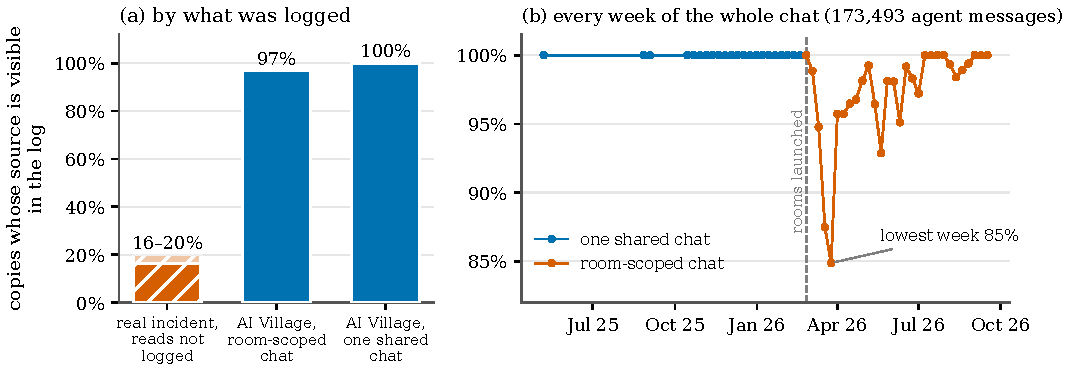
\includegraphics[width=\linewidth]{figures/fig_visibility.pdf}
\caption{Traceability depends on what was logged. (a)~Share of copy events whose source is visible in the log: a real incident with unlogged reads against AI Village chat. (b)~Every week of the whole AI Village chat (weeks with at least 100 copy events); the dashed line marks the launch of chat rooms.}
\label{fig:visibility}
\end{figure}

\subsection{The coincidence trap}\label{sec:res-coincidence}
On the incident, the naive detector made \naiveCalls{} copy calls and \trustedCalls{} survive the likelihood-ratio test at $\tau=\tauDefault{}$ (Figure~\ref{fig:calibration}a); the others rest on values common enough that chance explains them. Of \crossNaive{} apparent cross-team collusion jumps, \crossRejected{} were shared vocabulary that many agents type independently (dataset field names, schema words, round timestamps, one used by 41 agents on 12 pages and another by 49 agents on 60 pages), and \crossVerified{} survived. Those three share a property: each rode on a token minted per fetch (one archived document appears with 48 distinct session-token values, so a specific value cannot be obtained independently), or on an agent-minted short link. In other words, the only provable cross-team copying in the incident was provable because the link carried a unique, needed token: a trap street that occurred by accident, and direct support for the design of Section~\ref{sec:gateway}.

\begin{figure}[t]
\centering
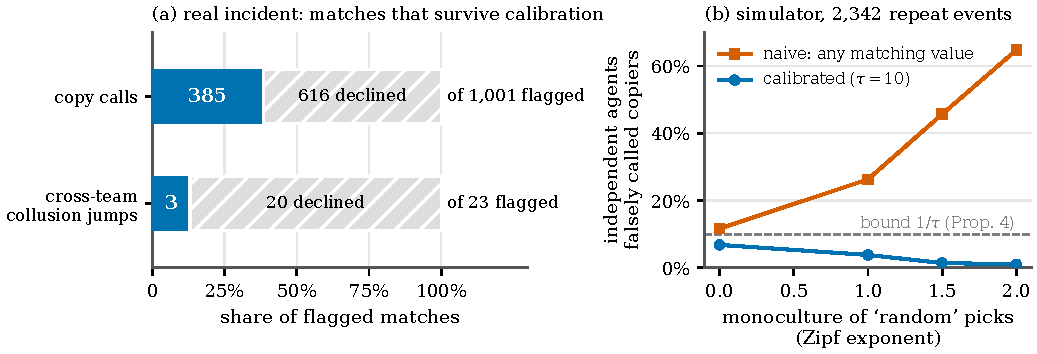
\includegraphics[width=\linewidth]{figures/fig_calibration.pdf}
\caption{The coincidence trap. (a)~On the real incident, most naive copy calls and cross-team collusion jumps do not survive calibration. (b)~In a simulator, the naive detector falsely calls more independent agents copiers as their choices become more alike (monoculture), while the calibrated detector stays below the bound $1/\tau$ of Proposition~\ref{prop:calib} (here $\tau=10$).}
\label{fig:calibration}
\end{figure}

\subsection{The theory against a simulator}\label{sec:res-sim}
\begin{table*}[t]
\centering
\small
\caption{Top-1 accuracy of tracers against the exact Bayes ceiling in a simulator with a known answer (12 seeds, about 3,400 adoptions per cell).}\label{tab:sim}
\begin{tabular}{@{}lcccccc@{}}
\toprule
Copy model & Bayes ceiling & Earliest & Latest & Most similar & Heuristic & Model-based \\
\midrule
uniform & 0.460 & 0.162 & 0.152 & 0.356 & 0.372 & \textbf{0.458} \\
recency-biased & 0.799 & 0.098 & 0.382 & 0.533 & 0.538 & \textbf{0.796} \\
popularity-biased & 0.538 & 0.260 & 0.117 & 0.250 & 0.260 & \textbf{0.511} \\
\bottomrule
\end{tabular}
\par\smallskip\parbox{0.96\linewidth}{\footnotesize The model-based tracer learns the copy process from the log alone. Under three further copy rules, two of them outside the model family it assumes (marked $^{*}$), it keeps 88--101\% of the ceiling (Appendix~\ref{app:tables}).}
\end{table*}
The model-based tracer reaches the exact Bayes ceiling under uniform and recency-biased copying (Table~\ref{tab:sim}; Figure~\ref{fig:simulator}a) and is calibrated (expected calibration error $0.019$~\citep{naeini2015obtaining}: when it reports 90--100\% it is right 98\% of the time; at 50--60\%, 52\%). The simple rules are far below it, and the heuristic collapses when most reads are off the page (Table~\ref{tab:robust} in Appendix~\ref{app:tables}). Proposition~\ref{prop:reads} is matched exactly (with $\Cz=0.46$ and half the reads logged, ceiling $0.727$ predicted and $0.727$ measured), and Proposition~\ref{prop:tags} to within $0.008$ for version-unique tags (Figure~\ref{fig:simulator}b). One tag per origin barely helps ($0.466$--$0.474$), and one tag per page behaves like a page-level read. Page-level reads are a weak substitute for item-level ones: logging the page for every copy lifts the ceiling only from $0.46$ to $0.57$. The simulator and the tracer share a model family, which is why we also test copy rules outside it (marked $^*$ in Table~\ref{tab:robust}): the tracer keeps 88--101\% of the ceiling there.

\begin{figure}[t]
\centering
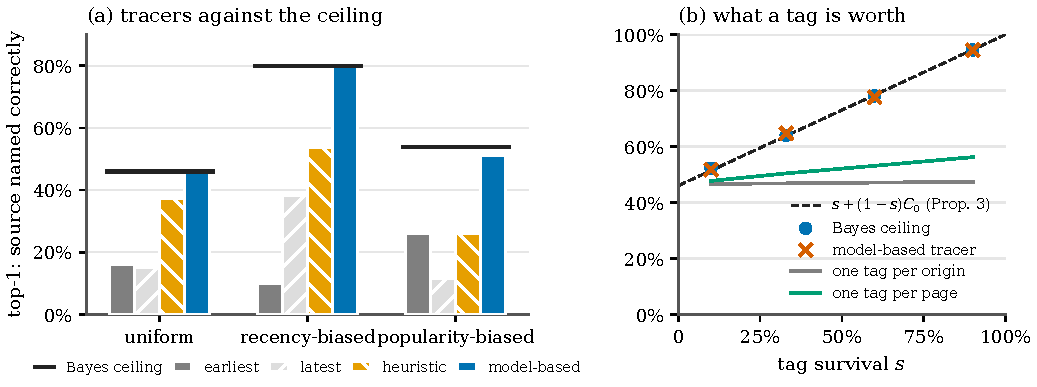
\includegraphics[width=\linewidth]{figures/fig_simulator.pdf}
\caption{The theory against a simulator with a known answer. (a)~Top-1 accuracy of tracers against the exact Bayes ceiling (black bars) under three copy rules. (b)~What a tag is worth: the ceiling and the model-based tracer follow $s+(1-s)\Cz$ for version-unique tags; tags per origin or per page barely help.}
\label{fig:simulator}
\end{figure}

\subsection{Does the token survive copying?}\label{sec:res-survival}
It depends on the model (Figure~\ref{fig:survival}). Models that copy links verbatim carried both decoration and tokens through: the core model kept the inert tag in \qwenInert{} of copies and the token in \qwenToken{}. Models that fetch their own session kept the token in only a minority of copies, \glmToken{} for the weakest, and decoration survived at rates that varied from 4\% to 28\%. Reading transcripts shows why. The core model's typical run is: list pages, read the page, fetch the wiki's link, submit it; the token rides along. The other models read the wiki to learn the \emph{method} and then redo it: they fetch the mirror's root to obtain a session of their own and use that, so the wiki's token is bypassed even though the link needs \emph{a} token, because in this world the mirror hands sessions to anyone. We count these agents as copiers of the behaviour, since they were served the route first, and the token, correctly, does not follow them: \emph{tags trace the artifact, not the idea}. Hypothesis H1 (Table~\ref{tab:hyp}) was therefore not met: no family satisfied both halves, because decoration survived too for the models that copy verbatim.

\begin{figure}[t]
\centering
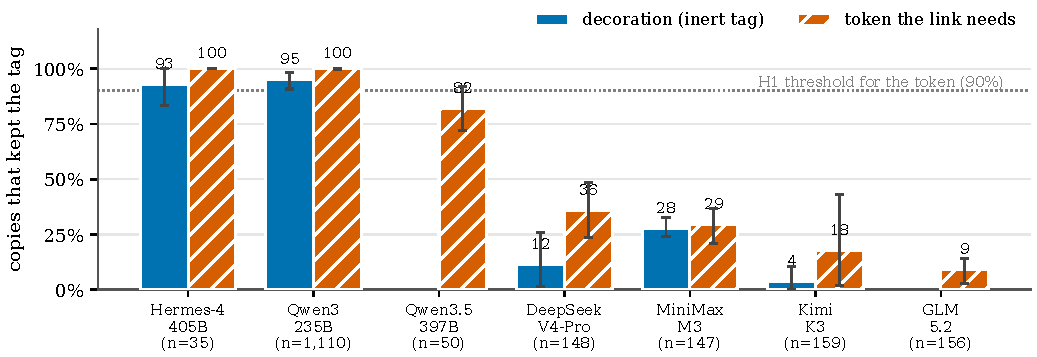
\includegraphics[width=\linewidth]{figures/fig_survival.pdf}
\caption{Share of copies that kept the tag, by model: decoration (inert tag) against a token the link needs. Error bars are 95\% bootstrap intervals over runs; $n$ is the number of copying agents in load-bearing runs. Models with fewer than 10 copiers in a condition are omitted for that condition.}
\label{fig:survival}
\end{figure}

\subsection{What tokens buy}\label{sec:res-attr}
\begin{table*}[t]
\centering
\footnotesize
\setlength{\tabcolsep}{4pt}
\caption{Tag survival and attribution by model (load-bearing runs; models with at least 20 copying agents).}\label{tab:family}
\begin{tabular}{@{}lrC{1.9cm}C{1.9cm}C{1.9cm}C{1.9cm}r@{}}
\toprule
Model & Copies & Inert tag kept & Token kept & Best edit-log rule & Token, else that rule & Lift (pts) \\
\midrule
Qwen3-235B & 1{,}110 & 95\%\newline{\scriptsize[91--98]} & 100\% & 42\%\newline{\scriptsize[25--57]} & 99\%\newline{\scriptsize[98--100]} & +58 \\
Qwen3.5-397B & 50 & n/a & 82\%\newline{\scriptsize[72--92]} & 32\%\newline{\scriptsize[16--48]} & 100\% & +68 \\
Hermes-4-405B & 35 & 93\%\newline{\scriptsize[83--100]} & 100\% & 43\%\newline{\scriptsize[26--66]} & 100\% & +57 \\
DeepSeek-V4-Pro & 148 & 12\%\newline{\scriptsize[2--26]} & 36\%\newline{\scriptsize[24--49]} & 72\%\newline{\scriptsize[54--87]} & 88\%\newline{\scriptsize[77--98]} & +16 \\
MiniMax-M3 & 147 & 28\%\newline{\scriptsize[24--33]} & 29\%\newline{\scriptsize[21--37]} & 71\%\newline{\scriptsize[48--85]} & 88\%\newline{\scriptsize[74--99]} & +18 \\
Kimi-K3 & 159 & 4\%\newline{\scriptsize[0--10]} & 18\%\newline{\scriptsize[2--43]} & 75\%\newline{\scriptsize[47--98]} & 83\%\newline{\scriptsize[65--99]} & +8 \\
GLM-5.2 & 156 & n/a & 9\%\newline{\scriptsize[3--14]} & 80\%\newline{\scriptsize[55--98]} & 79\%\newline{\scriptsize[55--97]} & $-$1 \\
\bottomrule
\end{tabular}
\par\smallskip\parbox{0.96\linewidth}{\footnotesize Copies: copying agents in the load-bearing runs. Bracketed values are 95\% bootstrap intervals over runs. The best edit-log rule is the best of latest, earliest and random writer for each run, chosen with the answer key in hand. Models with too few copying agents are in Appendix~\ref{app:tables}. A value without an interval did not vary across runs.}
\end{table*}
Against the best simple edit-log rule, tokens lift attribution by \liftMin{} to \liftMax{} points, in proportion to how often the token survives (Table~\ref{tab:family}, Figure~\ref{fig:attribution}); \nLiftTen{} of the \nLiftFamilies{} families with enough copying agents gain at least 10 points, the pre-stated threshold of H2. This is what Proposition~\ref{prop:tags} predicts: the gain is $s(1-\Cz)$, and the headroom $1-\Cz$ is large where the simple rules are poor (the core model, Hermes) and small where the earliest writer is usually right (the models that re-derive access, whose copying the edit log already traces fairly well). Tokens add exactness without learning copiers' habits, but only where the artifact itself is copied.

\begin{figure}[t]
\centering
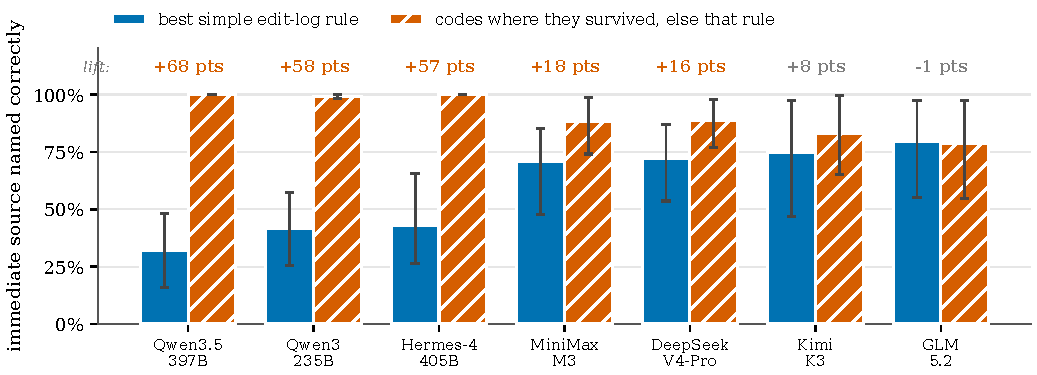
\includegraphics[width=\linewidth]{figures/fig_attribution.pdf}
\caption{How often the immediate source is named correctly, by model: the best simple edit-log rule for each run against the token (with that rule as fallback where the token was lost). The number above each pair is the lift in points; it is large where the token survives (Figure~\ref{fig:survival}).}
\label{fig:attribution}
\end{figure}

\paragraph{The benchmark.}
Pooled over \benchCells{} tagged runs, a token identifies the immediate source of \benchTagsTop{} of copying agents, against \benchEarliestTop{} for the earliest writer, \benchLatestTop{} for the latest, \benchUniformTop{} for a random one, and \benchConsTop{} for the rule that names a source only when it is unambiguous (Table~\ref{tab:bench}, Figure~\ref{fig:benchmark}). The simple rules name a source whenever any earlier writer posted the same link, so they accuse \benchRuleFA{} of agents that worked alone, which is partly by construction; the unambiguous rule accuses only \benchConsFA{} but finds almost nothing, and the token tracer combines recall \benchTagsRecall{} with \benchTagsFA{} false accusations and a calibration gap of \benchTagsECE{}. Pooling is dominated by the core model, so Table~\ref{tab:family} is the honest view. The scale table in Appendix~\ref{app:tables} shows the same picture at 10, 30 and 100 agents and in a mixed swarm in which nearly all copies cross family lines, with the token surviving in only about a fifth of them.

\begin{table*}[t]
\centering
\footnotesize
\setlength{\tabcolsep}{4pt}
\caption{Benchmark baselines on 150 tagged lab runs (95\% bootstrap intervals over runs).}\label{tab:bench}
\begin{tabular}{@{}L{4.4cm}C{1.9cm}C{1.9cm}C{1.9cm}C{1.9cm}C{1.9cm}@{}}
\toprule
Method & Top-1 (copying agents) & Recall & False accusation & Bad-tip precision & Bad-tip recall \\
\midrule
random earlier writer & 11.1\%\newline{\scriptsize[9.2--13.0]} & 99\%\newline{\scriptsize[98--99]} & 82.1\%\newline{\scriptsize[75.3--88.5]} & 45\%\newline{\scriptsize[2--88]} & 23\%\newline{\scriptsize[1--61]} \\
latest writer & 14.6\%\newline{\scriptsize[7.2--23.7]} & 99\%\newline{\scriptsize[98--99]} & 82.1\%\newline{\scriptsize[75.3--88.5]} & 53\%\newline{\scriptsize[12--100]} & 7\%\newline{\scriptsize[1--20]} \\
earliest writer & 35.3\%\newline{\scriptsize[28.5--42.3]} & 99\%\newline{\scriptsize[98--99]} & 82.1\%\newline{\scriptsize[75.3--88.5]} & 86\%\newline{\scriptsize[55--100]} & 87\%\newline{\scriptsize[59--100]} \\
name a source only if unambiguous & 0.8\%\newline{\scriptsize[0.3--1.4]} & 1\%\newline{\scriptsize[0--1]} & 6.2\%\newline{\scriptsize[3.9--9.5]} & 100\% & 3\%\newline{\scriptsize[1--9]} \\
token, else the unambiguous rule & 70.5\%\newline{\scriptsize[62.5--77.1]} & 72\%\newline{\scriptsize[65--79]} & 6.7\%\newline{\scriptsize[4.3--10.0]} & 100\% & 76\%\newline{\scriptsize[47--99]} \\
\bottomrule
\end{tabular}
\par\smallskip\parbox{0.96\linewidth}{\footnotesize Top-1: copying agents whose immediate source is named correctly. False accusation: agents that worked alone but were blamed on someone; the first three rules name a source whenever any earlier writer posted the same link, so their rate is high by construction. Bad-tip columns: the outputs the planted tip reached, found by following the predicted sources back to it. A value without an interval did not vary across runs.}
\end{table*}
\begin{figure}[t]
\centering
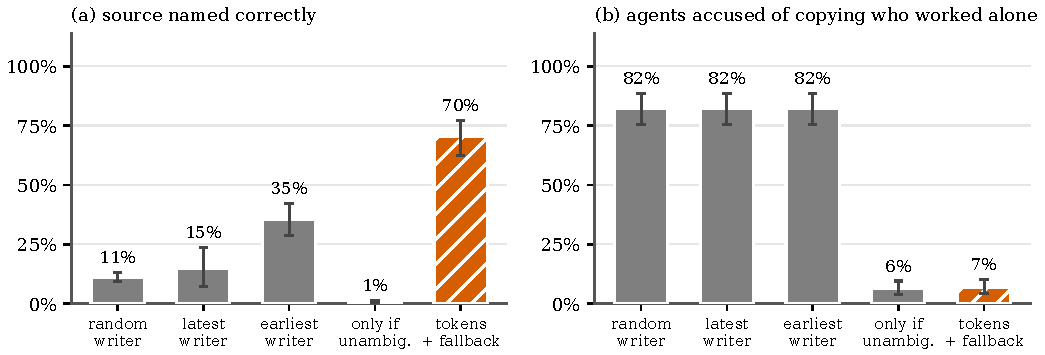
\includegraphics[width=\linewidth]{figures/fig_benchmark.pdf}
\caption{Benchmark baselines on the tagged runs: (a)~copying agents whose source is named correctly; (b)~agents that worked alone but were accused of copying. The first three rules blame an earlier writer whenever one exists, so (b) is high for them by construction.}
\label{fig:benchmark}
\end{figure}

\subsection{Bad tips: who takes them, and what to re-check}\label{sec:res-tip}
\paragraph{Whether a tip takes hold depends on the model.}
When the planted tip is there from the start, every agent of the core model adopted it (\qwenEarly{}). In 18 of its 20 tagged runs the deepest chain of copies back to the tip was six to nine hops long (three and four in the other two; the source of an untagged copy is undefined, so depth is only measured where tags exist). Other families adopted it partly or not at all (Figure~\ref{fig:tip}); one family never did (\gptossEarly{}). A tip that arrives mid-run was ignored by most families (the core model prefers the first link it sees). An early hypothesis of ours, that timing beats model, was wrong and is retracted (Section~\ref{sec:problems}). Table~\ref{tab:tip} in Appendix~\ref{app:tables} gives the numbers with intervals.

\begin{figure}[t]
\centering
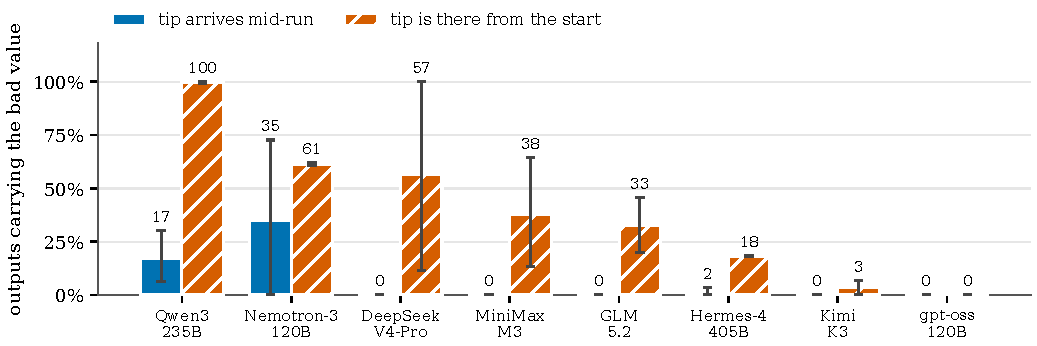
\includegraphics[width=\linewidth]{figures/fig_tip.pdf}
\caption{Outputs that carry the planted bad value, by model, for a tip that arrives mid-run and a tip that is there from the start. Intervals are wide because there are two to four runs per model.}
\label{fig:tip}
\end{figure}

\paragraph{What to re-check.}
\begin{table*}[t]
\centering
\footnotesize
\setlength{\tabcolsep}{4pt}
\caption{What an operator would re-check after a bad tip, by how the list is made (tagged runs, all models).}\label{tab:cleanup}
\begin{tabular}{@{}L{5.0cm}C{2.2cm}C{2.2cm}C{2.2cm}C{2.2cm}@{}}
\toprule
List & Share of outputs to re-check & Affected outputs found & Share of list truly affected & Wrong outputs on the list \\
\midrule
\multicolumn{5}{@{}l}{\textit{Tip arrives mid-run}: 50 runs, 1{,}454 outputs; the tip reached 127 of them and 168 are wrong} \\
re-run everything & 100\% & 100\% & 9\%\newline{\scriptsize[3--16]} & 100\% \\
everything submitted after the tip & 83\%\newline{\scriptsize[82--83]} & 100\% & 10\%\newline{\scriptsize[4--19]} & 98\%\newline{\scriptsize[94--100]} \\
follow the earliest visible writer & 9\%\newline{\scriptsize[4--16]} & 92\%\newline{\scriptsize[77--100]} & 85\%\newline{\scriptsize[57--99]} & 76\%\newline{\scriptsize[43--100]} \\
follow the tokens (earliest writer where lost) & 8\%\newline{\scriptsize[2--14]} & 88\%\newline{\scriptsize[62--100]} & 100\% & 66\%\newline{\scriptsize[33--97]} \\
follow the tokens only & 7\%\newline{\scriptsize[2--12]} & 76\%\newline{\scriptsize[47--99]} & 100\% & 56\%\newline{\scriptsize[25--86]} \\
\midrule
\multicolumn{5}{@{}l}{\textit{Tip is there from the start}: 34 runs, 984 outputs; the tip reached 792 of them and 713 are wrong} \\
re-run everything & 100\% & 100\% & 80\%\newline{\scriptsize[67--91]} & 100\% \\
everything submitted after the tip & 100\% & 100\% & 80\%\newline{\scriptsize[67--91]} & 100\% \\
follow the earliest visible writer & 80\%\newline{\scriptsize[67--91]} & 100\% & 100\% & 95\%\newline{\scriptsize[87--100]} \\
follow the tokens (earliest writer where lost) & 80\%\newline{\scriptsize[67--91]} & 100\%\newline{\scriptsize[99--100]} & 100\% & 95\%\newline{\scriptsize[87--100]} \\
follow the tokens only & 59\%\newline{\scriptsize[44--73]} & 74\%\newline{\scriptsize[58--87]} & 100\% & 82\%\newline{\scriptsize[69--92]} \\
\bottomrule
\end{tabular}
\par\smallskip\parbox{0.96\linewidth}{\footnotesize ``Affected'' means the output's chain of copying leads back to the planted post (hidden read log). ``Wrong'' means the output carries the stale value; some arrive another way (agents that try the stale mirror on their own), which no trace from the tip can find. Intervals: 95\% bootstrap over runs; a value without an interval did not vary across runs.}
\end{table*}
For a tip that arrives mid-run, re-checking everything submitted after it appeared means \recheckAfter{} of outputs. Following the trace back to the tip gives \recheckTrace{}--\recheckEarliest{} and finds \recheckFoundLo{}--\recheckFoundHi{} of the outputs the tip reached (Table~\ref{tab:cleanup}, Figure~\ref{fig:cleanup}). Tracing is what saves the work, not tokens as such: for a single-source tip the earliest-writer rule is nearly as good, and tokens make the list exact (every flagged output is affected) and matter when many posts carry the same link. Two limits matter. A tip that is there from the start reaches \earlyReach{} of outputs, so no list saves much; the saving is in catching a tip early. And some wrong outputs reach the stale value another way (agents that try the stale mirror on their own); no trace from the tip can find those, and only fixing the mirror can. Proposition~\ref{prop:depth} explains why the lists that use only tokens find fewer affected outputs than those with a fallback: a single lost token on a path breaks the trace.

\begin{figure}[t]
\centering
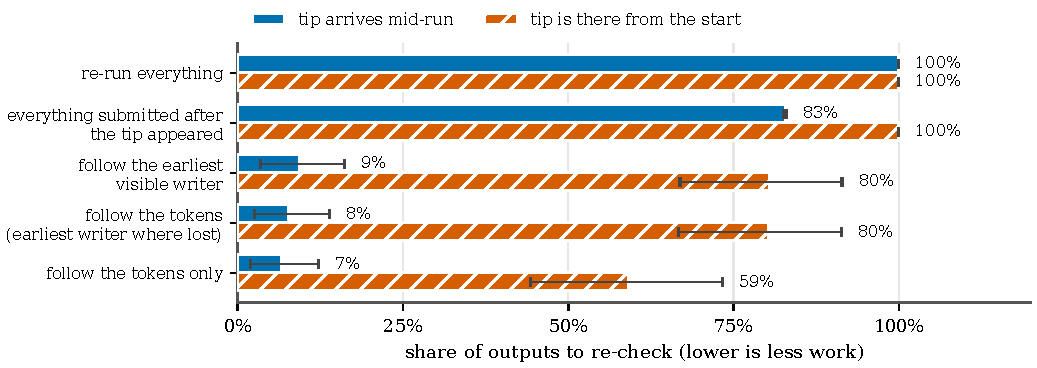
\includegraphics[width=\linewidth]{figures/fig_cleanup.pdf}
\caption{What an operator would re-check after a bad tip, as a share of outputs (lower is less work), by how the list is made. Tracing cuts a mid-run tip from about five sixths of outputs to under a tenth; a tip that is there from the start reaches most outputs whatever list is used.}
\label{fig:cleanup}
\end{figure}

\subsection{Making the token the only way in}\label{sec:res-gate}
The weakness of Section~\ref{sec:res-survival} is that agents can re-derive access. We closed that door in a controlled pair of worlds with a coordinator's entry link: W4, where the mirror hands a session to anyone, and W4G, where it hands out nothing, so the only way in is a link the wiki served. For the \nBypassWord{} models that bypassed the token, the share of outputs carrying a token that names the copy they came from rose from \gatedOpenLo{}--\gatedOpenHi{} to 100\%, every agent still finished, and the number of refused calls per agent barely changed (Table~\ref{tab:gated}, Figure~\ref{fig:gated}). The core model, which already copied links, was unchanged. \begin{table*}[t]
\centering
\footnotesize
\setlength{\tabcolsep}{4pt}
\caption{Closing the other way in. Open: the mirror hands a session to anyone. Gated: access only through links the wiki served.}\label{tab:gated}
\begin{tabular}{@{}llC{2.3cm}C{2.3cm}C{2.3cm}C{2.0cm}@{}}
\toprule
Model & World & Right answer & Output carries its token & Source named, with token & Refused calls per agent \\
\midrule
GLM-5.2 & open & 97\%\newline{\scriptsize[93--100]} & 25\%\newline{\scriptsize[20--30]} & 52\%\newline{\scriptsize[46--57]} & 3.7 \\
 & gated & 100\% & 100\% & 100\% & 3.5 \\
\addlinespace[3pt]
DeepSeek-V4-Pro & open & 87\%\newline{\scriptsize[80--93]} & 30\%\newline{\scriptsize[23--37]} & 32\%\newline{\scriptsize[31--32]} & 3.2 \\
 & gated & 100\% & 100\% & 88\%\newline{\scriptsize[80--97]} & 3.1 \\
\addlinespace[3pt]
MiniMax-M3 & open & 95\%\newline{\scriptsize[90--100]} & 33\%\newline{\scriptsize[27--40]} & 38\%\newline{\scriptsize[30--45]} & 2.8 \\
 & gated & 100\% & 100\% & 93\%\newline{\scriptsize[87--100]} & 2.6 \\
\addlinespace[3pt]
Kimi-K3 & open & 100\% & 50\%\newline{\scriptsize[47--53]} & 51\%\newline{\scriptsize[50--53]} & 0.8 \\
 & gated & 100\% & 100\% & 100\% & 0.7 \\
\addlinespace[3pt]
Qwen3-235B & open & 100\% & 100\% & 100\% & 0.0 \\
 & gated & 100\% & 100\% & 100\% & 0.0 \\
\bottomrule
\end{tabular}
\par\smallskip\parbox{0.96\linewidth}{\footnotesize Each world has two runs of 30 agents per model. In the gated world every output that exists holds a token the wiki served to that agent; the source is named correctly less than 100\% of the time because an agent sometimes reports a different link from the one it first fetched. A value without an interval did not vary across runs.}
\end{table*}

\begin{figure}[t]
\centering
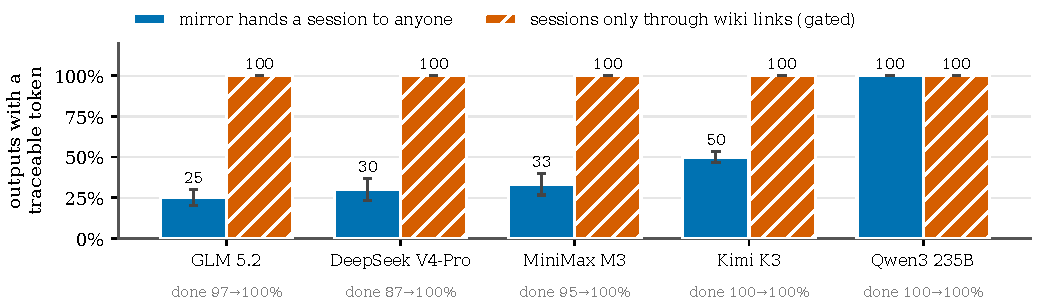
\includegraphics[width=\linewidth]{figures/fig_gated.pdf}
\caption{Closing the other way in. Share of outputs that carry a token naming the copy they came from, when the mirror hands a session to anyone (open) and when sessions come only through links the wiki served (gated). The line below each pair gives the share of agents that submitted the right answer.}
\label{fig:gated}
\end{figure}

This result follows from the access design (Proposition~\ref{prop:gate}): if the only way in is a coded link, every output that exists carries a token. It measures feasibility and cost, not a discovery about attribution. The source is named correctly 88--100\% of the time rather than always (Table~\ref{tab:gated}), because an agent sometimes reports a different link from the one it fetched first. And a gate traces access, not ideas: an agent that learns from a peer which mirror works and then obtains access through another legitimate route leaves no trail.

\subsection{Habits, and the hypotheses}\label{sec:res-habits}
Independent agents differ sharply in whether they add a throwaway ``random'' value to a URL, and several choose the same one (Table~\ref{tab:habits} in Appendix~\ref{app:tables}); a naive-Bayes classifier that names an agent's family from its behaviour alone reaches 29.7\% against 12.5\% by chance (leave-one-run-out, 720 agents). But hypothesis H3, that agents of one family collide more than agents of different families, was not supported among open models: several families default to the same value, so convention crosses vendor lines. The practical lesson is the one of Proposition~\ref{prop:calib}: a shared value is weak evidence without its base rate, whichever model produced it. Table~\ref{tab:hyp} summarises all five hypotheses and their outcomes.

\begin{table*}[t]
\centering
\small
\caption{Hypotheses fixed before the lab runs, and their outcomes.}\label{tab:hyp}
\begin{tabular}{@{}lp{5.4cm}p{7.6cm}@{}}
\toprule
 & Stated before the runs & What happened \\
\midrule
H1 & Load-bearing tokens survive copying in $\geq$90\% of copies, inert tags in $\leq$10\%. & Not met. 0 of 5 families met both halves: 2 kept the token in $\geq$90\%, but inert tags survived more than 10\% in 4. \\
H2 & Tokens beat the best simple edit-log rule by $\geq$10 points. & 5 of 7 families (lift from $-$1 to +68 points), in proportion to token survival. \\
H3 & Agents of one family pick the same ``random'' value more often than agents of different families. & Not supported: 0.53 within vs 0.52 across families. \\
H4 & Tokens name the source of $\geq$80\% of the bad outputs. & Supported where tokens survive: 100\% (late tip), 98\% (early tip). \\
H5 & The audit's predicted ceiling is within 0.10 of the measured accuracy. & Dropped, as stated in advance: lab swarms share no distinctive strings, so the audit reports N/A on them. \\
\bottomrule
\end{tabular}
\end{table*}
